\capitulo{5}{Aspectos relevantes del desarrollo del proyecto}
\section{Introducción}\label{cap:asp-rel}

En este capítulo se explicarán los aspectos más importantes tanto de la investigación como del desarrollo. Los detalles más específicos y los resultados obtenidos se encuentran en el \textit{Cuaderno de investigación} y los \textit{Anexos}. 

\section{Investigación}

La fase de investigación ha ocupado la mayor cantidad de tiempo de este proyecto ya que ha sido también una introducción a la carrera investigadora. Ha sido desarrollada conjuntamente con Alicia Olivares Gil bajo la dirección de nuestros tutores el Dr. Álvar Arnáiz González y el Dr. José Francisco Díez Pastor.

El comienzo de esta investigación comenzó con un estudio del arte con el fin de conocer métodos y soluciones ya existen y se han probado. Sin embargo, la mayoría de artículos que existen actualmente para ese problema se centran en datos de encefalogramas, un tipo de datos que no poseemos. También exploramos problemas semejantes como detecciones de caídas mediante sensores de presión aunque la mayoría de estos sistemas se basaban en otros sensores como cámaras o acelerómetros. Algunos de estos artículos están resumidos en la sección~\ref{cap:trabrel}.

Tras esta exploración bibliográfica nos centramos en el estudio de los datos. Primero haciendo una limpieza eliminando datos con poca variabilidad, normalizarlos y eliminar datos ruidosos. Tras esto generamos proyecciones de los mismos a dos dimensiones tanto con datos limpiados, estadísticos o filtrados.

Los datos estadísticos que generamos en un comienzo fueron medias y desviaciones móviles de ventana $25$. Los filtros tratados fueron el \textit{butterworth} y el \textit{savgol}, ambos de la librería \textit{SciPy}~\cite{tool:scipy}.

Las primeras conclusiones que obtuvimos era que los datos intermedios de las crisis documentadas tenían ciertas propiedades que las diferenciaba del resto, sin embargo esto se perdía aumentando la ventana del estudio. Además que este proceso era muy lento y necesitaba una gran cantidad de datos por lo cual realmente podíamos obtener si hubo una crisis y no hacer una detección en directo.

A partir de aquí, para facilitar los procesos de preprocesado se crearon un conjunto de transformadores de datos que incluyen un normalizador por característica como por grupos de las mismas, un filtro de ruido, un eliminador de características de poca varianza, un calculador de estadísticos móviles, un modificador del valor objetivo según una ventana temporal y dos compuestos que concatenan resultados o los convierte en una línea de tuberías de tal forma que se ejecuten secuencialmente.

Antes de pasar a la exploración de métodos para clasificar, acotamos las duraciones de las crisis que nos habían reportado, la primera razón es que la misma empresa nos informó de que los datos eran estimados y estos superaban el umbral para \textit{status epilepticus}~\cite{epilepsia}. Esta acotación se hizo analizando manualmente los datos dentro del rango que nos dieron determinando como crisis las situaciones con presiones anómalas. 

\subsection{Detección de anomalías}
Lo siguiente que se realizó fue un estudio de detección de anomalías en el cual se intentó tanto predecir una crisis a partir de entrenar un clasificador \texttt{OneClassSVM} entrenando con todos los datos de no crisis y también predecir una situación de no crisis entrenando el mismo clasificador con los datos de crisis.

Lo primero que obtuvimos es que una crisis es un subconjunto de una situación no crisis ya que el clasificador no lo detecta como anomalía al ser entrenado con las situaciones de no crisis.

El segundo obtenido fue que las diversas crisis no coexisten en el mismo espacio, ya que al entrenar el clasificador con una crisis determinaba como anomalía a todas las demás crisis al igual que al resto de datos. Además, en el caso de combinar dos situaciones de crisis el entrenamiento ya tiene un gran índice de fallo si los datos no son estadísticos (media y desviación).

Los resultados del entrenamiento se pueden ver en las tablas~\ref{tab:matriz-conf-1a} y~\ref{tab:matriz-conf-1a-2d} y lo de test en las tablas~\ref{tab:matriz-test-2a} y~\ref{tab:matriz-test-3a}, en estás últimas se puede ver que la predicción siempre es errónea para un conjunto nuevo de datos.

\myinput{./research-book/train-tables.tex}
\myinput{./research-book/test-tables.tex}

\subsection{\textit{Ensembles} para desequilibrados}
Debido a que la detección de anomalías no dio resultados correctos se pasó a hacer un estudio de clasificadores combinados (\textit{ensemble}) optimizados para la resolución de problemas con datos desequilibrados~\cite{diez2015diversity,galar2012review}.

Debido a que el conjunto de datos ya habíamos hecho un submuestreo al limitar el conjunto de datos a los del día de las crisis probamos a hacer un sobremuestreo mediante SMOTE~\cite{galar2012review} con los algoritmos de \textit{Bagging}, \textit{AdaBoostM1} y \textit{Rotation Forest}~\cite{rodriguez2006rotation}.

Los resultados de este experimento fue que los clasificadores sobreajustaban los datos de las crisis y no eran capaces de predecir correctamente otras crisis. Además pudimos comprobar que el algoritmo de \textit{boosting} no predecía correctamente los datos de entrenamiento lo que, junto con el hecho de que la etiquetación sabíamos que había sido manual, da pie a la conclusión de que los datos están mal etiquetados~\cite{ubu:mineria3}.

También se probó a realizar una validación cruzada con todo el conjunto de datos usando el clasificador de \textit{Rotation Forest}~\cite{rodriguez2006rotation} obteniendo unos buenos resultados.

\subsection{Búsqueda de mejores características}
Otro proceso que se hizo fue la búsqueda de mejores características a partir de un análisis estadístico tratando a los datos como una serie temporal. A partir primero de la búsqueda de la mejor ventana temporal (obtenido el valor de noventa) mediante la optimización del valor del AUC~\cite{galar2012review} y de PRC~\cite{Davis2006RPR}. El desarrollo completo de esta búsqueda está mejor explicado en el Apéndice \textit{Cuaderno de Investigación} en el capítulo \textit{Extracción de características con tsfresh y clasificador Random Forest}.

\subsection{\textit{Ensembles} para desequilibrados - estadísticos de series temporales}
Para finalizar la investigación se volvieron a probar los \textit{ensembles} para conjuntos desequilibrados de Galar et. al.~\cite{galar2012review} y Díez et. al.~\cite{diez2015random, diez2015diversity} usando sobremuestreo con \textit{SMOTE}, submuestreo con \textit{RUS} y muestreo aleatorio con \textit{Random Balance}. Se usaron los clasificadores de comité aleatorio, \textit{bagging} y \textit{rotation forest}.

Los resultados fueron semejantes a la primera ocasión ya que el testeo con la otra crisis siempre obtenía un ratio de aciertos con las crisis de 0.

Los resultados se pueden ver en las tablas~\ref{tab:crisis1} y~\ref{tab:crisis2}

\begin{table}\scriptsize
	\begin{center}
		\begin{tabular}{llllllll}
			\toprule
			{} & TPR &          FPR &       TNR & FNR &       PRC &       AUC &       ACC \\
			\midrule
			RB - Bag                &   0 &            0 &         1 &   1 &  0.984425 &  0.552363 &   0.98178 \\
			RB - RC       &   0 &            0 &         1 &   1 &  0.981267 &  0.485675 &   0.98178 \\
			RB - RotF        &   0 &  1.65036e-06 &  0.999998 &   1 &  0.980551 &  0.485354 &  0.981778 \\
			RUS - Bag          &   0 &  0.000899444 &  0.999101 &   1 &  0.980613 &  0.447139 &  0.980897 \\
			RUS - RC &   0 &            0 &         1 &   1 &  0.981076 &    0.4806 &   0.98178 \\
			RUS - RotF  &   0 &  0.000394435 &  0.999606 &   1 &  0.982287 &  0.486412 &  0.981393 \\
			SM - Bag                         &   0 &  0.000173287 &  0.999827 &   1 &  0.984367 &  0.565807 &   0.98161 \\
			SM - RC                &   0 &            0 &         1 &   1 &  0.981278 &  0.486071 &   0.98178 \\
			SM - RotF                 &   0 &  1.56784e-05 &  0.999984 &   1 &  0.982673 &  0.512364 &  0.981764 \\
			\bottomrule
		\end{tabular}
		\caption{Métodos para desbalanceados - Entrenamiento con la primera crisis, testeo con la segunda crisis.}
		\label{tab:crisis1}
	\end{center}
\end{table}

\begin{table}\scriptsize
	\begin{center}
		\begin{tabular}{llllllll}
			\toprule
			{} & TPR &         FPR &       TNR & FNR &       PCR &       AUC &       ACC \\
			\midrule
			RB - Bag                &   0 &   0.0109634 &  0.989037 &   1 &  0.995225 &  0.491511 &  0.983616 \\
			RB - RC       &   0 &  0.00571683 &  0.994283 &   1 &  0.993912 &  0.446135 &  0.988834 \\
			RB - RotF        &   0 &  0.00488364 &  0.995116 &   1 &   0.99517 &  0.525534 &  0.989663 \\
			RUS - Bag          &   0 &   0.0461306 &  0.953869 &   1 &  0.994863 &  0.514533 &  0.948642 \\
			RUS - RC &   0 &   0.0112769 &  0.988723 &   1 &  0.994602 &  0.506568 &  0.983304 \\
			RUS - RotF  &   0 &   0.0128567 &  0.987143 &   1 &  0.994482 &  0.468075 &  0.981733 \\
			SM - Bag                         &   0 &    0.017596 &  0.982404 &   1 &  0.995505 &  0.539099 &   0.97702 \\
			SM - RC                &   0 &   0.0048424 &  0.995158 &   1 &  0.994052 &  0.458383 &  0.989704 \\
			SM - RotF                 &   0 &  0.00344412 &  0.996556 &   1 &  0.994742 &  0.502318 &  0.991094 \\
			\bottomrule
		\end{tabular}
		\caption{Métodos para desbalanceados - Entrenamiento con la segunda crisis, testeo con la primera crisis.}
		\label{tab:crisis2}
	\end{center}
\end{table}

\section{Desarrollo de la aplicación}
La fase de desarrollo ha ocupado alrededor de un cuarto del tiempo del proyecto. A su vez se ha dividido en cuatro partes: una primera de búsqueda de herramientas para la difusión en tiempo real de datos, una segunda de diseño, una tercera de implementación y finalmente el despliegue.

La primera parte fue la más corta, consistió en explorar herramientas que fueran compatibles con websocket~\cite{wiki:websocket} ya que este protocolo es el más eficaz para distribución en tiempo real de datos mediante HTTP, que es la tecnología más sencilla para la creación de una \textit{API}. La herramienta seleccionada fue \textit{socketIO}~\cite{tool:socketio} que daba una interfaz sencilla y multilenguaje.

\subsection{Diseño}
La fase de diseño fue la que más tiempo llevó de este apartado ya que hubo que discutir muchos detalles con mi compañera Alicia Olivares, ya que se debía crear una interfaz sencilla y funcional para que pudiese desarrollar una aplicación Android lo más rápidamente posible.

El primer paso fue determinar los casos de uso, que debido a la limitación temporal, se resumieron lo más posible. Decidimos hacer una gestión de usuarios y camas con un sistema de permisos simplificado de forma tal que los usuarios pueden estar asociados a camas. También se creó un usuario maestro administrador que tuviese permisos sobre todo.

Otro punto importante fueron los datos. Los usuarios son formados por un identificador único, un nombre de usuario único, una contraseña y un token dinámico y único. Este último es el que permite identificar al usuario para realizar operaciones \textit{CRUD}. Este cambia por cada inicio de sesión del usuario de tal forma que solo puede existir una sesión abierta a la vez.

Las camas, por otro, lado están formadas por un par de identificadores de los sensores de presión (\textit{MAC}) y de los sensores biométricos (\textit{UUID}) que son usados también como el nombre del espacio donde se difundirán los datos de esa cama. También identifican a la cama un número secuencial y un nombre de la misma. Cada cama tiene a su vez una combinación de IP-puerto del rango de \textit{multicast} que especifica a la aplicación a donde tiene que escuchar. 

Como parte final del diseño se determinó cuales serían los pasos para el \textit{handshake} del proceso de obtención de datos en tiempo real. Se decidió que este sería una petición a la API para solicitar el espacio de nombres, luego una apertura de conexión a \textit{socketIO}, si la conexión era correcta lanzar una petición de solicitud de datos (\texttt{give\_me\_data}) para finalmente escuchar paquetes (\texttt{package}) al espacio de nombres solicitado.

\subsection{Implementación}
El último proceso fue la implementación, que se dividió en cuatro partes: primero la creación de la \textit{API REST} para la gestión de camas y de usuarios, la segunda fue la implementación de la difusión de datos en tiempo real, la tercera la creación de ventanas para la interacción vía web y por último la creación de test unitarios y de integración (interfaz).

\subsubsection{Implementación de la \textit{API}}
Esta \textit{API} se implementó utilizando dos partes, una primera como una clase \textit{singleton} que sirve de conexión a la base de datos y realiza las operaciones especificadas controlando los permisos y una segunda parte que hace de adaptador para traducir peticiones \textit{HTTP} a la signatura de las funciones de la clase.

El funcionamiento global de una petición es:
\begin{enumerate}
	\item Se hace una petición \texttt{POST} mediante \texttt{x-www-form-urlencoded} a la ruta de la operación deseada.
	
	\item La función asociada a la ruta desempaqueta el mensaje y crea una llamada al objeto de la \textit{API}.
	
	\item La \textit{API} realiza la operación solicitada y devuelve el resultado deseado.
	
	\item La función de adaptación recoge el resultado y crea un objeto de respuesta \textit{JSON} con un código \textit{HTTP} y un mensaje.
\end{enumerate}

En el caso de que alguno de los procesos fallasen, se generaría un código de error según el tipo de error. Si fuese 400 implicaría que la petición realizada no tiene los parámetros esperados, 401 si el valor del \textit{token} no está correctamente asociado, 403 si no se tuviesen permisos para realizar la operación, 404 si no existiese la operación deseada, 405 si se hace con un método erróneo, 418 si la operación no estuviese disponible por causa de la versión y 500 en el caso de que existiese un error en el servidor. Si todo fuese correcto el número del código sería 200. Todos estos valores provienen del estándar RFC~7231~\cite{RFC7231}.

\subsubsection{Difusión en tiempo real}
Para poder hacer la difusión en tiempo real se necesita de la librería de \texttt{flask-socketio}~\cite{tool:flask-socketio} y de \texttt{gevent}~\cite{tool:gevent}. 

El primer paso es crear los hilos del \textit{pipeline} del procesamiento de los datos (uno de escucha y otro de procesado). Esto se hace usando la interfaz \texttt{Thread} pero compatibilizado con \texttt{gevent} mediante un \textit{mokey patching}~(explicado en la sección~\ref{cap:mokey}).

El proceso completo de creación de hilos se puede ver en el Anexo \textit{Manual del programador}, la estructura de su colaboración se puede ver en el diagrama de clases de la figura~\ref{fig:classes}.

\begin{figure}
	\centering
	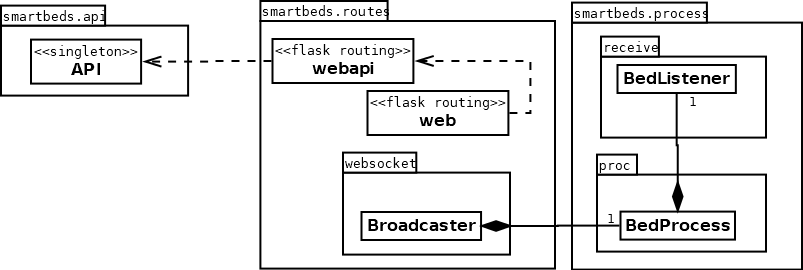
\includegraphics[width=\textwidth]{classes}
	\caption{Diagrama de clases.}
	\label{fig:classes}
\end{figure}

Tras esto es necesario crear las capturas de eventos de \textit{socketIO} para poder detectar cuando se solicitan datos y enviarlos. Este envío se hace mediante otro hilo, el de difusión que emite por \textit{broadcast} a todos los clientes de cada cama. Estos hilos funcionan solo dentro del entorno de petición (\textit{request context}) por lo que morían al cerrar el usuario la conexión, por tanto, para evitar que los datos se acumulasen en el servidor se usaron colas en los hilos de procesamiento con un tamaño máximo a la ventana temporal~(90) de tal forma que se borrasen los más viejos si entraban nuevos datos.

Un detalle importante es que como los datos no podemos tenerlos en tiempo real, ya que pertenecen a la empresa que nos los suministra. Por ello hemos simulado un \textit{streaming} de datos local usando UDP emitiendo una nueva linea del CSV cada $0.4$ segundos, que es una estimación del intervalo por el cual nos llegan los datos.

Otra modificación sobre el diseño ha sido que realmente existe una única cama y las distintas camas que existen realmente usan los mismos hilos ya que los \textit{Broadcaster} realmente emiten a todos los \textit{namespaces} que existen. Se ha hecho esto debido a las limitaciones técnicas del equipo de despliegue ya que cada cama implicaba una serie de tres hilos que ralentizan mucho el sistema.

También se utiliza actualmente un clasificador aleatorio por intervalos de tal manera que cambie la probabilidad de crisis cada noventa instancias entre los tres estados posibles: crisis, no crisis, despierto; con el fin de poder probar como cambian las interfaces en los distintos estados, sobre todo porque el clasificador obtenido al final no era capaz de predecir situaciones de crisis.

El resultado final en la aplicación web se puede ver en la figura~\ref{fig:man_bed}

\begin{figure}
	\centering
	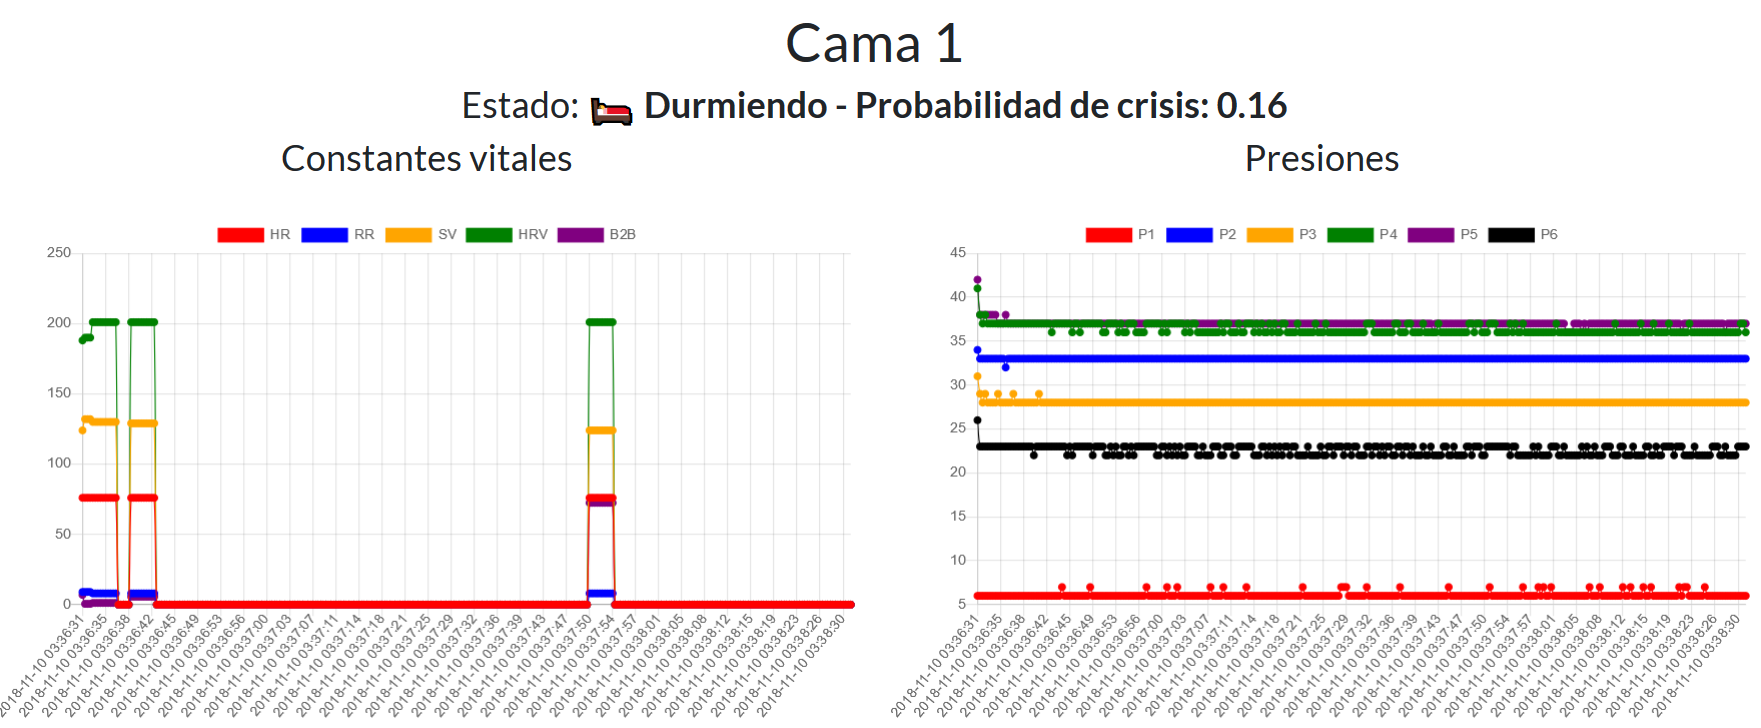
\includegraphics[width=\textwidth]{manual/man_cama1}
	\caption{Página con la información en tiempo real de una cama.}
	\label{fig:man_bed}
\end{figure}


\subsubsection{Ventanas \textit{HTML}}

La interfaz web de la aplicación se hizo mediante plantillas \textit{Jinja}~\cite{tool:jinja} de \textit{HTML}. Se apoyó con el \textit{framework} de \textit{boostrap 4}~\cite{wiki:boostrap} para el \textit{CSS} y \textit{jQuery} para la implementación de funciones \textit{JavaScript}.

Para facilitar este desarrollo se crearon varios componentes separados y una plantilla maestra de la que heredarían todas las páginas. Esto evita el código repetido así como facilita el desarrollo de la aplicación. Los componentes que se crearon fueron la barra de navegación, el pie de página, las funciones generales de para la validación de los formularios y un modal para mostrar los errores.

Otro aspecto importante del desarrollo de la interfaz fue la creación de los gráficos en tiempo real. Se usó la librería \textit{Graph.js} para hacer gráficos en objetos \texttt{canvas} de \textit{HTML}. En un primer momento la librería actualizaba muy lentamente, pero el problema estaba en la programación de los hilos de \textit{Python} con los hilos, esto se solucionó con la llamada \texttt{eventlet.sleep(0)} en el \texttt{Broadcaster} para que los datos fuesen en tiempo real.

Para optimizar el renderizado es estas gráficas se optó por eliminar las animaciones y los valores de \texttt{hover}\footnote{Evento al estar el puntero del ratón sobre el objeto} para que no se ejecutasen nuevas llamadas a eventos del \texttt{DOM} que mostraban los datos de esa instancia temporal.

Otra tecnología que se usó en el desarrollo de la interfaz web fue el uso de llamadas asíncronas al servidor mediante \textit{AJAX}. De esta manera se pueden evitar cargas completas de la página de manera innecesaria. Especialmente en las situaciones que la operación no requería mostrar nuevos datos en la pantalla como la creación, modificación o borrado de usuarios y camas. 

\subsubsection{Pruebas}
Las pruebas consistieron en pruebas unitarias y de integración. Para las primeras se usó \texttt{unnittest} de \textit{Python} y para las de integración se hicieron test sobre la interfaz web con \textit{Selenium IDE}. Este por motivos de tiempo no se ha trasladado a código y se puede ejecutar importando el fichero .side al \textit{IDE} y ejecutarlo desde el mismo. En el Anexo \textit{Manual del Programador} este punto está más explicado.

Los test unitarios se basaron en un test parametrizado y un fichero \textit{JSON} con la configuración de todos los test deseados.
\\\\ %Para no dejar viudas
\begin{lstlisting}[language=JSON]
{
   "tests": [
      {
         "name": "nombre del test",
         "description": "descripcion del test",
         "func": "funcion de la clase API",
         "input": ["parametros de entrada en orden"],
         "output": ["salida esperada"],
         "excepts": "excepciones esperadas, si es null no se espera ninguna"
      },
      ...
   ],
   "tokens": 
      {
         "usuario": "token",
         ...
      }
}
\end{lstlisting}

Cada test tiene seis campos, un nombre y descripción para identificar al test, una función de la clase \texttt{smartbeds.api.API}, una entrada en el orden de los parámetros, la salida esperada (si espera una) y la excepción que espera (si espera una). También tiene una serie de tokens asociados a los usuarios, aunque ese campo es solamente útil para el programador de los test para saber que token está asociado a cada usuario.

Antes de ejecutar los tests se instala una base de datos de pruebas que borra la base de datos anterior.

\subsection{Despliegue}
El despliegue de la aplicación fue una de las partes más complicadas del proceso de desarrollo. En primer lugar se intentó desplegar sobre un dispositivo embebido, en particular la \textit{Raspberry Pi 2B}. Sin embargo, este \textit{hardware} no fue capaz de soportar el rendimiento necesario para enviar los datos en un tiempo real.

Por eso se traspasó el sistema a otro servidor personal\footnote{Este servidor forma parte del grupo \textit{JKA Network}} con varias máquinas virtuales llamado \textit{Al-Juarismi}. Se incorporó la base de datos a una de ellas de nombre \textit{V-Lovelace} y la lógica de la aplicación se almacenó en la máquina \textit{V-Babbage}. En esta última también se añadió la simulación de la cama como un demonio semejante al que se puede ver en el anexo del \textit{Manual del programador}. %TODO: incorporar características de las máquinas virtuales.

Este servidor está configurado de tal forma que se requiera un certificado \textit{SSL} sobre todas las páginas que albergue. Por tanto se usó un certificado de \textit{LetsEncrypt} para el mismo.

\section{Test de usabilidad}

Para comprobar si la aplicación web realizada era usable e intuitiva se realizó un test de usabilidad junto a la aplicación móvil realizada por Alicia Olivares Gil. Para comprobar eso se propusieron cinco tareas a los usuarios:

\begin{enumerate}\small
	\item Iniciar sesión con el usuario y contraseña que te hemos proporcionado. 
	\item Cambiar tu contraseña (ten en cuenta que una vez cambies tu contraseña deberás usar la nueva en cualquiera de las dos aplicaciones). 
	\item Consultar el estado de los pacientes. 
	\item Consultar las gráficas explicativas sobre el estado de los pacientes. 
	\item Cerrar sesión	
\end{enumerate}

Y para recoger las valoraciones se pidió la cumplimentación de un formulario con cuatro afirmaciones a valorar entre 1 y 5 siendo 1 \textit{completamente en desacuerdo} y 5 \textit{completamente de acuerdo}. Las afirmaciones eran:
\begin{itemize}\small
	\item \textit{Me ha resultado fácil realizar las tareas propuestas}.
	\item \textit{Me ha resultado fácil interpretar los elementos gráficos (iconos, botones, gráficas...)}.
	\item \textit{La selección de elementos gráficos usados en la aplicación (colores, tipografías...) me ha parecido acertada}.
	\item \textit{La aplicación me ha parecido muy buena}.
\end{itemize}

A estas afirmaciones, para facilitar la interpretación de los resultados, se les ha asignado una valoración equivalente cuyos nombres han sido: \textit{Facilidad de uso}, \textit{Interpretabilidad}, \textit{Uso de gráficos} y \textit{Global} respectivamente.

También se hizo una distinción entre el perfil profesional del encuestado entre \textit{tecnológico}, \textit{educación} y \textit{asistencia sanitaria}. El objetivo de esta distinción es poder comprobar si la aplicación es fácil de usar por el tipo de usuario al que va destinado (educadores y asistentes sanitarios). Se ha tomado como referencia las valoraciones de los usuarios de perfil técnico. 

\subsection{Resultados del test}
Ha habito un total de doce votos, cinco de perfil tecnológico y tres de educación y cuatro de asistencia sanitaria (Fig.~\ref{fig:usab_prop})

\begin{figure}
	\centering
	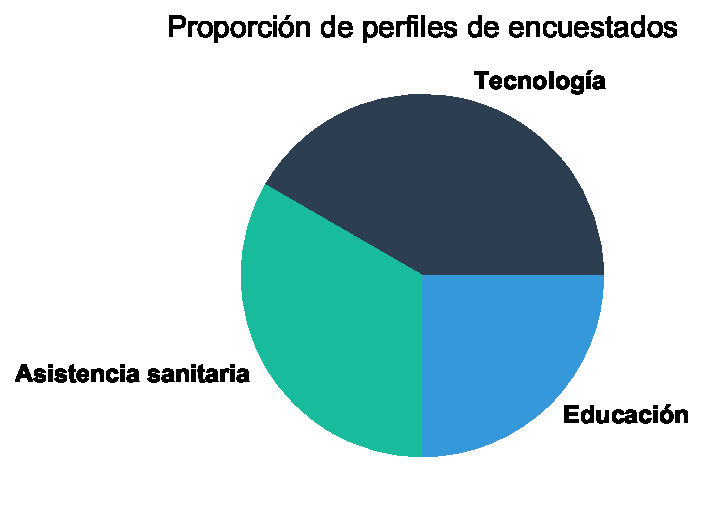
\includegraphics[width=0.6\textwidth]{usability/web_proportion.pdf}
	\caption{Proporción de encuestados según su perfil laboral}
	\label{fig:usab_prop}
\end{figure}

Podemos ver en la figura~\ref{fig:usab_global} las valoraciones generales de todos los encuestados. Podemos ver que la valoración general es muy positiva. La interpretabilidad de los datos es lo que peor calificación tiene, podemos observar que existen algunas valoraciones muy bajas sobre este punto, aún así la media es de $3.5$ que sigue por encima de la neutralidad de la valoración, podemos concluir que la aplicación es usable e intuitiva.

\begin{figure}
	\centering
	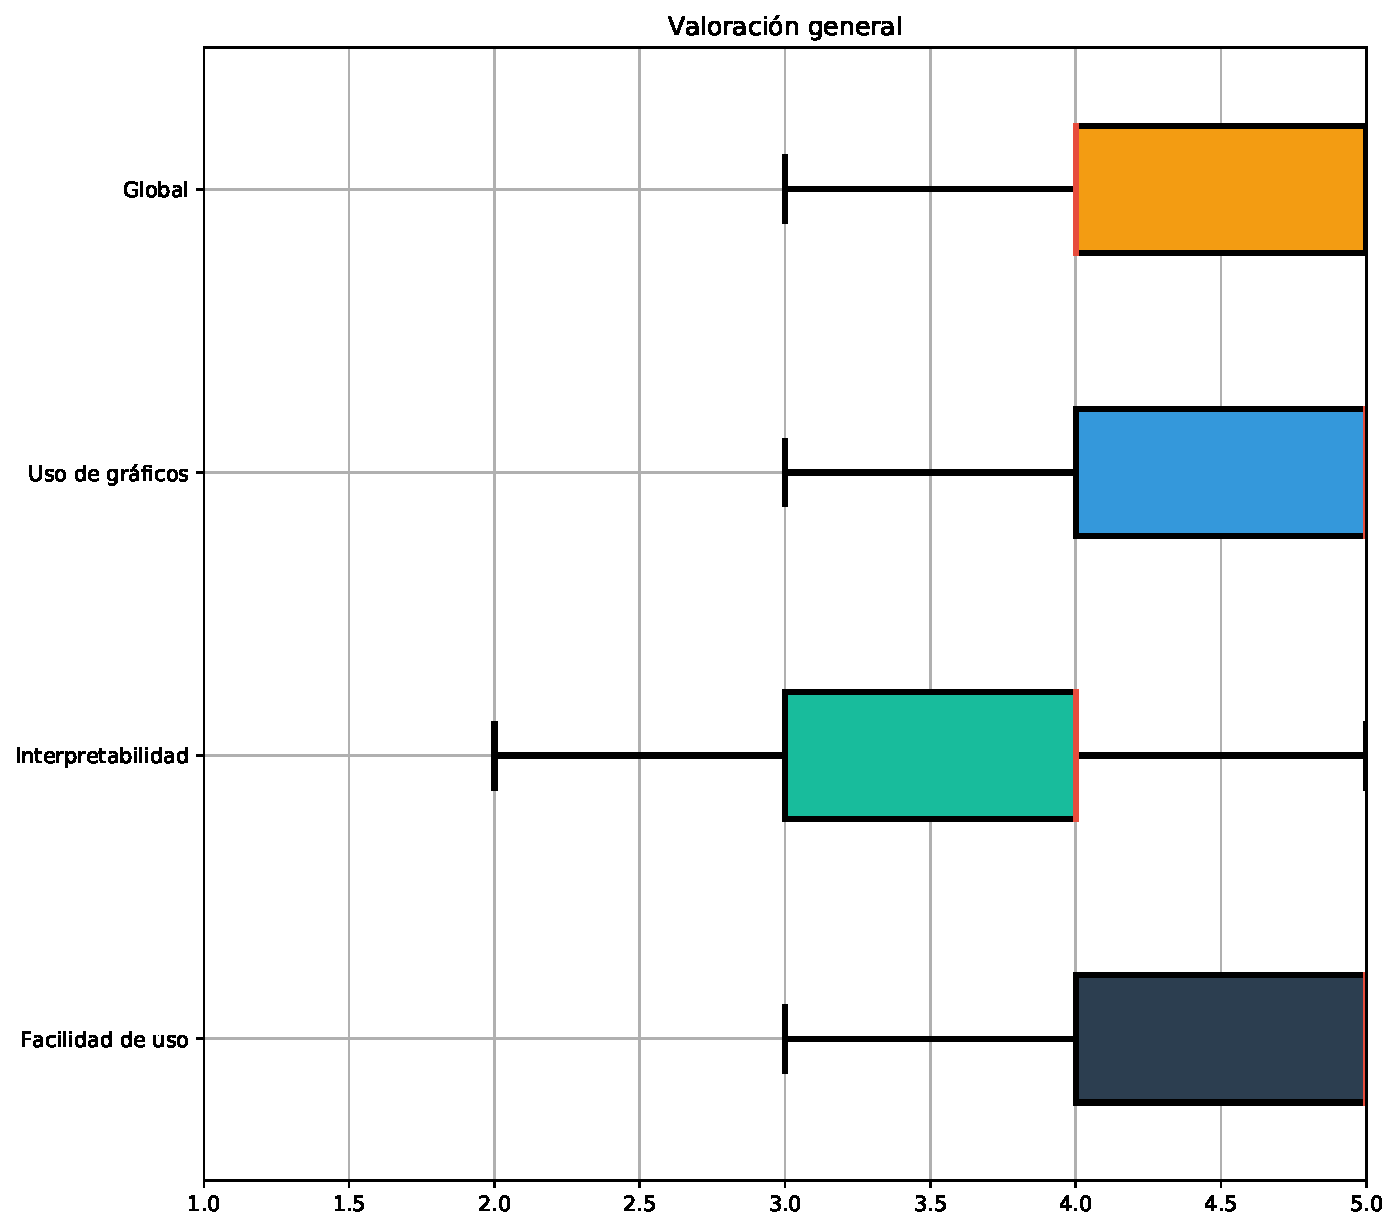
\includegraphics[width=\textwidth]{usability/web_general.pdf}
	\caption{Valoraciones de todos los encuestados}
	\label{fig:usab_global}
\end{figure}

Respecto a la comparativa entre el perfil \textbf{tecnológico} y el \textbf{no tecnológico} (Fig.~\ref{fig:usab_comp} podemos observar que, aunque la valoración global y la interpretabilidad por los usuarios \textbf{no tecnológico}s están más dispersas siguen teniendo valores medios muy altos. Además, sus valoraciones tanto sobre el uso de gráficos como de la facilidad de uso es menos dispersa que la del grupo \textbf{tecnológico}.

Por todo esto podemos concluir que la aplicación es usable e intuitiva para el perfil al que está destinado y no ha habido ninguna tendencia en el desarrollo de hacer una aplicación excesivamente técnica que hubiese perjudicado la usabilidad de la misma.

\begin{figure}[h]
	\centering
	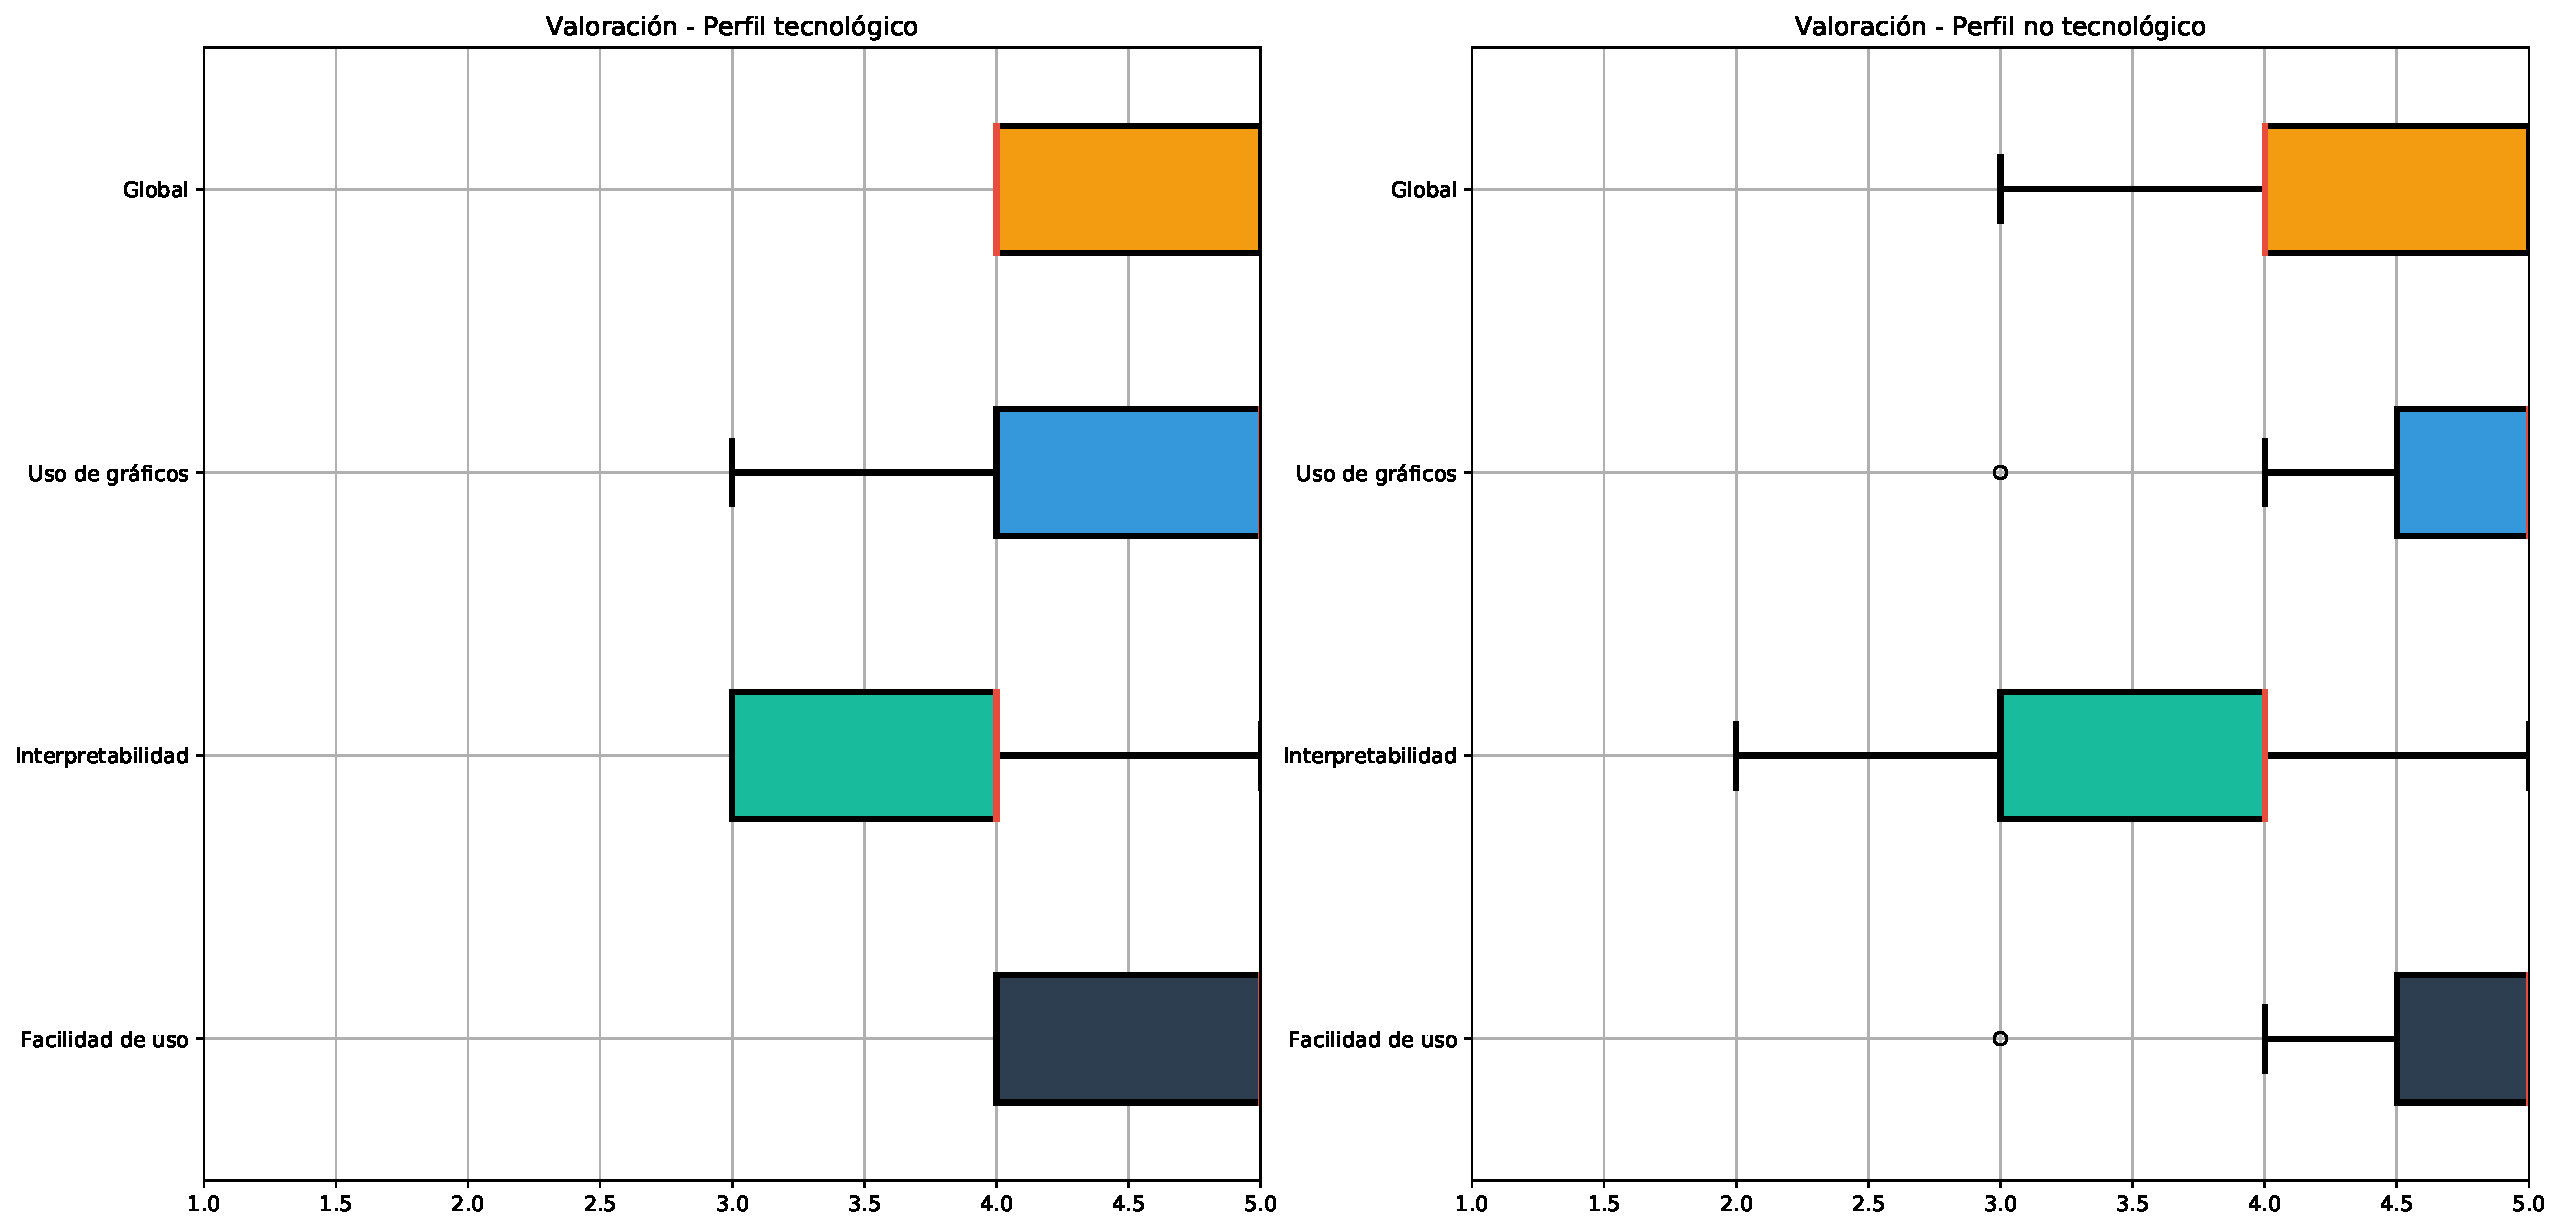
\includegraphics[width=\textwidth]{usability/web_comparation.pdf}
	\caption{Comparación de valoraciones entre perfil tecnológico y no tecnológico}
	\label{fig:usab_comp}
\end{figure}

\section{\textit{Mokey Patching}}\label{cap:mokey}

También conocido como el parches de mono en español, es la técnica por la cual se extiende o modifica la funcionalidad del sistema de manera local y en ejecución. Solo se permite en lenguajes dinámicos como \textit{Python} o \textit{Ruby}~\cite{wiki:monkey_patch}.

Bajo esta definición las librerías \textit{Gevent}~\cite{tool:gevent} y \textit{Eventlet}~\cite{tool:eventlet} aportar una función de parcheo para cambiar las funciones de las librerías nativas de \textit{Python}: \texttt{sockets}, \texttt{dns}, \texttt{time}, \texttt{select}, \texttt{thread}, \texttt{os}, \texttt{ssl}, \texttt{httplib}, \texttt{subprocess}, \texttt{sys}, \texttt{aggresive}, \texttt{Event}, \texttt{builtins}, \texttt{signal} y \texttt{queue}.

Gracias a esto todas esas funciones y clases que no son compatibles con el sistema de eventos de \textit{socketIO} se pueden utilizar sin necesidad de aprender todas las funciones y clases alternativas de \textit{gevent} o \textit{eventlet}.

\section{Uso de \textit{CodeClimate}}
Para hacer un estudio de la calidad del código y hacer las modificaciones necesarias para que el código sea más mantenible, se ha utilizado \textit{CodeClimate} una herramienta que analiza gratuitamente proyectos de \textit{GitHub} de código abierto.

En el primer análisis se obtuvo una calificación de \textbf{\textit{F}}, siendo la peor nota posible. Sin embargo, esto fue debido a que se analizó partes del proyecto que no es propio como son las librerías de \textit{JavaScript} y los estilos \textit{CSS} que se han utilizado. Por ello se creó un fichero \texttt{.codeclimate.yml} para ignorar todo el código ajeno y se volvió a realizar un análisis.

El segundo análisis tuvo de calificación \textit{\textbf{C}}, que aunque no es la peor calificación, si que requiere una mejora del código para hacerlo más mantenible. Para ello se eliminó código repetido, que en su mayoría trataba de comprobaciones de la validez de las llamadas a las funciones (comprobación de tipos y de la sesión web). Para solucionar esto se incluyeron funciones que agrupasen las comprobaciones idénticas eliminando así el código repetido.

Una situación especial fue la creación de un \textit{decorador} para las funciones de las rutas de la web para que se ejecutase en todas las que se requiriese la inclusión del \texttt{token} del usuario en la sesión actual para poder redirigir correctamente estas peticiones. 

La última ejecución se obtuvo una calificación de \textit{\textbf{B}}. A partir de este punto es difícil de mejorar debido a que algunos errores detectados no son refactorizables. Estos son la gran cantidad de parámetros de algunas funciones, que no pueden ser modificadas al ser heredadas de otras librerías; la cantidad de métodos de la clase \texttt{API} que, al englobar toda la lógica de negocio, no tiene sentido partir en diferentes clases. 
